\documentclass[a4paper]{article}
\usepackage[utf8]{inputenc}
\usepackage[T2A]{fontenc}
\usepackage[12pt]{extsizes}

\usepackage[english,russian]{babel}
\usepackage[left=10mm, top=10mm, right=10mm, bottom=20mm, nohead, nofoot]{geometry}
\usepackage{amsmath,amsfonts,amssymb} % математический пакет
\headsep=10mm

\usepackage[most]{tcolorbox} % для управления цветом
% НАСТРОЙКИ
%теорема
\definecolor{theorem-color}{gray}{0.90} % уровень прозрачности (1 - максимум)
\newtcolorbox{htheorem}{colback=theorem-color,grow to right by=-4mm,grow to left by=-4mm,
    boxrule=0pt,boxsep=0pt,breakable} % настройки области с изменённым фоном

%определение
\definecolor{def-color}{gray}{0.98}
\newtcolorbox{definit}{colback=def-color,grow to right by=-4mm,grow to left by=-4mm,
    boxrule=0pt,boxsep=0pt,breakable} % настройки области с изменённым фоном

%доказательсвто теоремы
\definecolor{proof-color}{gray}{0.95} % уровень прозрачности (1 - максимум)
\newtcolorbox{hproof}{colback=proof-color,grow to right by=-1mm,grow to left by=-1mm,
    boxrule=0pt,boxsep=0pt,breakable} % настройки области с изменённым фоном

%замечания, следствия
\definecolor{consectary-color}{gray}{0.95} % уровень прозрачности (1 - максимум)
\newtcolorbox{cns}{colback=consectary-color,grow to right by=-4mm,grow to left by=-4mm,
    boxrule=0pt,boxsep=0pt,breakable} % настройки области с изменённым фоном



\usepackage{fancybox,fancyhdr}
\pagestyle{fancy}
\fancyhf{}
\fancyhead[R]{ФТ-104}
\fancyfoot[R]{\thepage}
\fancyhead[L]{Матанализ}

\usepackage{hyperref}
\hypersetup{colorlinks=true, allcolors=[RGB]{010 090 200}} % цвет ссылок 
\newcommand{\lr}[1]{\left({#1}\right)} % команда для скобок

\title{Конспектик к экзамену по алгему}
\author{Васильев Павел}
%\linespread{1}
\usepackage{amsmath}

\usepackage{graphicx}
\usepackage{ifpdf}
\ifpdf
\DeclareGraphicsRule{*}{mps}{*}{}
\fi
\usepackage{graphicx}
\usepackage{color}
\graphicspath{ {images/} }

\begin{document}
\section*{Исследование функций с помощью старших производных. Выпуклость функции. Асимптоты.}


\begin{htheorem}
	\textbf{Теорема}. Пусть $\exists f^{(n)} (x_0) \neq 0, n \geq 2$ и $\forall i \in (1, ..., n-1) f ^{(n)} = 0$.
	
	Тогда 
	\begin{enumerate}
	\item Если $n$ чётное:
		\begin{enumerate}
		\item если $f^{(n)} (x_0)>0 \Rightarrow x_0$ - точка локального минимума
		\item если $f^{(n)} (x_0)<0 \Rightarrow x_0$ - точка локального максимума
		\end{enumerate}

	
	\item Иначе экстремума нет, но:
	\begin{enumerate}
	\item Если $f^{(n)} (x_0)>0 \Rightarrow f$ строго возрастает
	\item Если $f^{(n)} (x_0)<0 \Rightarrow f$ строго убывает
	\end{enumerate}
		\end{enumerate}
\end{htheorem}

\begin{hproof}
\textbf{Доказательство.}

Посмотрим на формулу Тейлора с остаточным членом в форме Пеано:

\begin{equation}
\displaystyle f(x) = f(x_0) + \sum_{k=1}^n \frac{f^{(k)} (x_0)}{k!} (x-x_0)^k + o((x-x_0)^n)
\end{equation}

Поскольку по условию $\displaystyle \forall i \in (1, ..., n-1) f ^{(n)} = 0$, то $\sum_{k=1}^n \frac{f^{(k)} (x_0)}{k!} (x-x_0)^k = \frac{f^{(n)} (x_0)}{n!} (x-x_0)^n$

$f(x) = f(x_0) + \frac{f^{(n)} (x_0)}{n!} (x-x_0)^n + o((x-x_0)^n)$

Перенесём $f(x_0)$ влево и посмотрим на знак $f(x) - f(x_0)$: $f(x) - f(x_0) = \frac{f^{(n)} (x_0)}{n!} (x-x_0)^n + o((x-x_0)^n), x \rightarrow x_0$

\begin{enumerate}
\item $n$ чётное:

$(x-x_0)^n > 0, n!>0 \Rightarrow$ знак выражения $\displaystyle \frac{f^{(n)} (x_0)}{n!} (x-x_0)^n$ определяет $f^{(n)} (x_0)$, при этом $o((x-x_0)^n)$ не влияет на знак, потому что это бесконечно малая величина.

Поэтому если $f^{(n)} (x_0) > 0$, то $\displaystyle \frac{f^{(n)} (x_0)}{n!} (x-x_0)^n > 0 \Rightarrow f(x) - f(x_0) > 0$ - локальный минимум.

Аналогично если $f^{(n)} (x_0) < 0$, то $f(x) - f(x_0) < 0$ - локальный максимум.

\item $n$ нечётное:

У $\displaystyle \frac{f^{(n)} (x_0)}{n!} (x-x_0)^n$ величина $\displaystyle \frac{f^{(n)} (x_0)}{n!} > 0$. 

Если $x < x_0$, то $(x-x_0)^n < 0 \Rightarrow f(x) - f(x_0) < 0$.
Если $x > x_0$, то $(x-x_0)^n > 0 \Rightarrow f(x) - f(x_0) > 0$.
Следовательно если $f^{(n)} (x_0) > 0$, то $f$ возрастает в $x_0$, если $f^{(n)} (x_0) < 0$, то $f$ убывает в $x_0$ $\blacksquare$
\end{enumerate}

\end{hproof}

\subsection*{Выпуклость функции на промежутке}

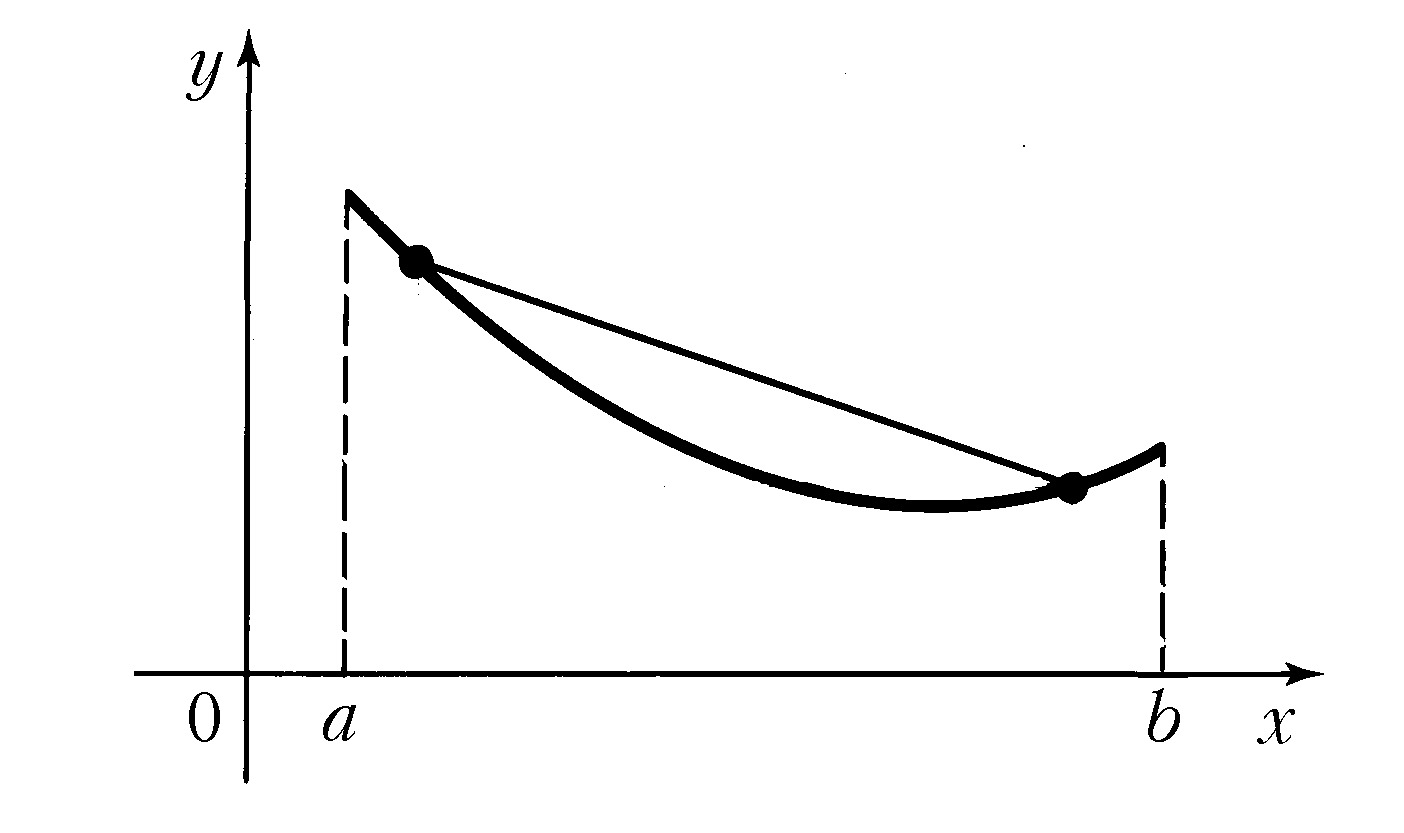
\includegraphics[scale=1.3]{images/convex_function.jpg}

Пусть $f(x)$ определена на $[a, b]$.Возьмём две точки $x_1, x_2 \in [a,b], x_1, x_2$ и обозначим за $l(x)$ хорду, соединяющую $f(x_1)$ и $f(x_2)$.

Тогда $f$ \textbf{выпуклая} на $[a,b]$ если $\forall x_1, x_2: a \leq x_1 < x_2 \leq b: \forall x \in (x_1, x_2): f(x) \leq l(x)$

\begin{htheorem}
\textbf{Теорема}. $f$ выпукла на $[a,b]$ $\Leftrightarrow$ надграфик ($\{(x, y): x \in [a,b]$ и $y \geq f(x)\}$) - выпуклое множество.
\end{htheorem}

\begin{hproof}
\textbf{Доказательство.}

Доказательство самостоятельно.
\end{hproof}

Давайте выведем уравнение прямой $l(x)$.

$l(x)$ имеет коэффициент, равный отношению $\displaystyle \frac{f(x_2)-f(x_1)}{x_2-x_1}$, а в точке $x_1$ имеет значение, равное $f(x_1)$. Тогда $l(x) = \displaystyle \frac{f(x_2)-f(x_1)}{x_2-x_1} x + f(x_1)$


\begin{htheorem}

Пусть $f$ дважды дифференцируема на $[a, b]$. Тогда $f''(x) \geq 0, x \in [a,b] \Rightarrow f$ выпукла.
\end{htheorem}

\begin{hproof}
Хотим, чтобы $f(x) - l(x) \leq 0 \quad \forall x \in [a,b]$.

$\displaystyle f(x) - \frac{f(x)(x-x_2) + f(x_2)(x_1-x)}{x_1-x_2} = \frac{f(x)(x_1-x_2) - f(x_1)(x-x_2) - f(x_2)(x_1-x)}{x_1-x_2} = \\ = \frac{f(x)((x_1-x)+(x-x_2)) - f(x_1)(x-x_2) - f(x_2)(x_1-x)}{x_1-x_2} = \\ = \frac{(f(x) - f(x_1))(x-x_2) + (f(x)-f(x_2))(x_1-x)}{x_1-x_2} = \\ = \{ \text{Используем теорему Лагранжа} \} = \frac{(x-x_2)f'(\xi)(x-x_1) - (x-x_1)f'(\eta)(x-x_2)}{x_1-x_2}$ \\ (здесь $\xi \in [x_1, x], \eta \in [x, x_2]$, то есть $\xi < \eta$) $ = \displaystyle \frac{(x-x_2)(x-x_1)f''(\tau)}{x_1-x_2}, \tau \in [\xi, \eta]$

Теперь посмотрим на выражение $\displaystyle \frac{(x-x_2)(x-x_1)f''(\tau)}{x_1-x_2}$

$(x-x_1)>0, (x-x_2)<0, x_1-x_2 < 0, f''(\tau) \leq 0, \xi - \eta < 0 \Rightarrow$ всё выражение $\leq 0$.

\end{hproof}

\begin{htheorem}\textbf{Теорема (без доказательства)}.

Выпуклая функция непрерывна на $(a,b)$.

Во всех точках $(a,b)$ есть $f_-', f_+'$.

\end{htheorem}

\textbf{Определение.} Точка $x_0$ - точка перегиба у $f$, если в левой и правой окрестностях $x_0$ функция имеет разный характер выпуклости.

\begin{htheorem}
Пусть $f$ дважды непрерывно дифференцируема ($f''$ непрерывна) на $[a,b]$. Тогда если $x_0 \in (a,b)$ - точка перегиба, то $f''(x_0) = 0$.

\end{htheorem}

\begin{hproof}\textbf{Доказательство.}
От противного.

Если $f''(x_0) > 0$ и $f''$ непрерывна, то в $O(x_0)$ сохраняется знка, то есть $f(x) > 0 \quad \forall x \in O(x_0) \Rightarrow f$ выпуклая вниз в $O(x_0)$, что противоречит тому, что $x_0$ - точка перегиба.

Аналогично доказываем от противного когда $f''(x_0) < 0$. $\blacksquare$

\end{hproof}

\subsection*{Асимптота}

\textbf{Определение.} Говорят, что $y(x) = kx + b$ \textbf{асимптота} для $f(x)$ при $x \rightarrow \pm \infty$, если $\displaystyle \lim_{x \rightarrow \pm \infty} (f(x) - kx - b) = 0$

Говорят, что $y(x) = kx + b$ \textbf{асимптота} для $f(x)$ при $x \rightarrow a$, если $f(x) \rightarrow \infty$ при $x \rightarrow a$.

\subsubsection*{How to найти асимптоту?}

Получим необходимое условие на $k$.

$\displaystyle \lim_{x \rightarrow +\infty} (f(x) - kx - b) = 0 \Leftrightarrow \lim_{x \rightarrow +\infty} (f(x) - kx) = b \Rightarrow \lim_{x \rightarrow +\infty} \left( \frac{f(x)}{x} - k \right) = \frac{b}{\infty} = 0$

$\displaystyle \lim_{x \rightarrow +\infty} \left( \frac{f(x)}{x} - k \right) = \frac{b}{\infty} = 0 \Leftrightarrow \lim_{x \rightarrow +\infty} \frac{f(x)}{x} = k$. Найдём $k$. Затем найдём $b$ из $\displaystyle \lim_{x \rightarrow +\infty} (f(x) - kx) = b$.
\end{document}
